%%%%%%%%%%%%%%%%%%%%%%%%%%%%%%%%%%%%%%%%%%%%%%%%%%%%%%%
% A template for Wiley article submissions.
% Developed by Overleaf. 
%
% Please note that whilst this template provides a 
% preview of the typeset manuscript for submission, it 
% will not necessarily be the final publication layout.
%
% Usage notes:
% The "blind" option will make anonymous all author, affiliation, correspondence and funding information.
% Use "num-refs" option for numerical citation and references style.
% Use "alpha-refs" option for author-year citation and references style.

\documentclass[alpha-refs]{wiley-article-04t}
% \documentclass[blind,num-refs]{wiley-article}

% Add additional packages here if required
\usepackage{siunitx}

% For figures
\usepackage{graphics}

%For captions - even though template has complex caption commands
\usepackage[labelfont=bf,justification=centering]{caption}
\usepackage[font=small,labelfont=bf]{subcaption}
\captionsetup[sub]{font=small,labelfont={bf,sf}}

%% For figures numbered by section
\usepackage{chngcntr}
\counterwithin*{figure}{section}
\counterwithin*{table}{section}


%% For figure numbers rolling



%% Additional links for hyperref
\usepackage[unicode=true,pdfusetitle,
 bookmarks=false,bookmarksnumbered=false,bookmarksopen=true,bookmarksopenlevel=2,
 breaklinks=false,pdfborder={0 0 1},backref=false,colorlinks=false]
 {hyperref}
\hypersetup{pdfstartview={XYZ null null 1}}

\usepackage[backend=bibtex,
			natbib=true, 
			style=chicago-authordate]{biblatex}
\addbibresource{Returns.bib}

\usepackage{array}
\usepackage{longtable}
%\usepackage{fullpage}

\usepackage{lmodern}
\newcommand{\graph}[3]{
\raisebox{-#1mm}{\includegraphics[height=#2em,width=3cm]{#3}}
}

\usepackage{booktabs} % for vertically partitioned table

\usepackage{lipsum}  % for fillers

% Additional
\usepackage{amsmath}
\usepackage{tabularx}
\usepackage{tabulary}
\usepackage{float}
\usepackage[flushleft]{threeparttable}

\usepackage[export]{adjustbox} % for figure in frame


\usepackage{array}
\newcolumntype{L}[1]{>{\raggedright\let\newline\\\arraybackslash\hspace{0pt}}m{#1}}
\newcolumntype{C}[1]{>{\centering\let\newline\\\arraybackslash\hspace{0pt}}m{#1}}
\newcolumntype{R}[1]{>{\raggedleft\let\newline\\\arraybackslash\hspace{0pt}}m{#1}}

%%%%%%%%#################################################################################%%%%%%%%%%%%%%%%%%%%%%%%%%%%%


% Update article type if known
\papertype{WORLD BANK EDUCATION GLOBAL PRACTICE}
% Include section in journal if known, otherwise delete
\paperfield{Russian Federation: Analytical Services and Advisory Activity: 
P170978}

\title{Skills and Returns to Education in the Russian Federation: Policy Note}

\author[]{}

\runningauthor{P170978:Skills and Returns to Education in the Russian 
Federation: Policy Note  \hspace{6em} \today}


\acks{\begin{normalsize}
\emph{Country Director:} Renaud Seligman; \emph{Regional Director:} Fadia 
Saadah; \emph{Practice Manager:} Harry Patrinos; \emph{Program Leader:} 
Dorota Nowak; \emph{Peer Reviewers}: Cristian Aedo; Ruslan Yemtsov; Husein 
Abdul-Hamid; \\ \textbf{Team:} Harry Patrinos; Suhas Parandekar; Ekaterina 
Melianova; Art\"{e}m Volgin; Polina Zavalina; Zhanna Terlyga. 

\end{normalsize}}




\usepackage[framemethod=tikz]{mdframed}

\begin{document}

\maketitle
\vspace{-2.5cm}


\section{Main Messages}

\vspace{-0.5em}

\begin{mdframed}[hidealllines=true,backgroundcolor=blue!20]

	
\hspace{-1em}  \textbf{Objective:} 

%\textcolor{blue!20}{Blix}
\begin{small}
\phantom{0}
\end{small}

\vspace{-1em}

\hspace{-2.2em} The objective of this ASA was ``to develop policy 
recommendations for the 
Russian Federation based on a detailed analysis of the returns to education 
and identification of feasible pathways for robust growth in Russia's human 
capital wealth''. The second part of identifying feasible pathways was 
perhaps stated too ambitiously. The study does include elements of possible 
future strategy work with priority regions as well as a potentially very 
useful idea for individual universities and colleges. 
\vspace{0.5em}

\hspace{-2.8em}  \textbf{Findings:} 

\vspace{-1em}
\begin{enumerate}
\item Returns to Education increased in the beginning of the 2000s but then 
started to decline to reach about 8\% now, below the EU average of 10\%; 
Part of this tendency can be explained by post-schooling depreciation of 
human capital.

\item Female returns to schooling higher than males.

\item Returns to education vary widely across region, with policy	
implications for economic development, especially for ten high priority 
depressed regions.

\item Matching data about graduate earnings and college and university 
costs is currently viable and can be very useful for potential students and 
to incentivize quality improvements for tertiary education institutions.
\end{enumerate} 

\vspace{-1em}

\hspace{-2.8em}  \textbf{Recommendations:} 
\vspace{-1em}
\begin{enumerate}

\item \textit{Education quality and innovation policy:} The Russian 
Federation needs to make investments in the quality of education and 
enhance youth entrepreneurship to stem the tide of falling returns to 
education.

\item \textit{Policy needs to work harder for gender parity:} Gender 
earning gaps remain wide and can be solved through policies to retain 
women?s interest in university education and learning opportunities at work.

\item \textit{Lifelong learning for vocational education:} Supporting 
continuous investment in human capital through the career is more important 
now the base level of education in Russia is amongst the highest in the 
world; this will reduce depreciation, especially for vocational education.

\item \textit{Strategy for priority regions:} A policy diagnostic based 
even on rough measures of labor market demand and supply is shown to 
capture regional diversity; refine the measures further for high priority 
regions to arrive at customized policy solutions, for example for three 
pilot regions of Pskov Oblast, Altai Krai and the Adygea Republic.


\item \textit{Government transparency for citizen benefit:}. Revitalize the 
\href{https:\\graduate.edu.ru}{graduate.edu.ru} website which has not 
been updated since 2016; Deepen the financial information collected from 
\href{https:\\bus.gov.ru}{bus.gov.ru} and annually update resulting data on 
institution level education returns to  improve student choice and system 
efficiency.

\end{enumerate} 

	
\end{mdframed}

\newpage

\section{Motivation}


The motivation for this study is to provide inputs to the development 
strategy of the Russian Federation as set out in the May decree of 2018. 
Russia's development goal is to become one of the top five economies in 
the world and to reduce poverty by half. The importance of human capital to 
reach this goal is recognized in the government's policy pronouncements and 
the World Bank analytical work in support of government policy. 
A recently published World Bank study reported that Human capital  only 
accounts for 46\% of total wealth in Russia, as compared to the OECD 
average of 70\% \parencite{Naikal2019}. The report showed that even as 
growth rates of per capita  wealth was ten times higher in Russia as 
compared to OECD, the gap in levels with OECD is still very wide. The per 
capita human capital wealth  level at average for the OECD in 2014 was 
about USD 500,000 \textendash  five times that of Russia's 95,000 (measured 
in  2014 dollars). In order to catch up faster with the OECD, returns to 
education  in Russia will need to be increased. This requires an 
understanding of the trends regarding the returns to education across time 
and across the considerable spatial diversity of the Russian Federation. 

\vspace{1em}

\noindent\fbox{%
	\parbox{0.99\textwidth}{%
According to the Human Capital Index (HCI), the Russian Federation scores 
at 538 points in the Harmonized Learning Outcomes (HLO) global indicator, 
which is close to the advanced attainment and places Russia in the top-ten 
countries in terms of learning outcomes, though on the overall HCI, Russia 
is ranked 34th out of 157 countries. The Human Capital Index (HCI) measures 
the amount of human capital that a child born today can expect to attain by 
age 18 \parencite{kraay2018}. The HCI shows that a child born in the Russian 
Federation today will be 73\% as productive when she grows up as she could 
be if she enjoyed complete education and full health 
\parencite{worldbank2019}. In contrast to the excellent 
research focused on learning outcomes, this  study is focused on the period 
after the age of 18, examining the empirical record of the labor market.  
	}%
}


\vspace{1em}


This study is based on four working papers. Working Paper 1 and 
Working Paper 3 of the study seek to meet the analytical need to understand 
the temporal and spatial patterns in the returns to education. The time 
trend described for the period 1994-2018 in Working Paper 1 requires an 
explanation. Moving beyond the traditional view of higher 
educational attainment of the population resulting in declining returns, 
Working Paper 2 explores the role played by depreciation of human capital. 
Working Paper 1 also indicates that individuals are responsive to changes 
in the returns of education, and that the proportion of women choosing 
university education has slightly declined in recent years. Working Paper 4 
investigates more closely the institutional level returns to education, 
albeit with a limited short-term horizon of three years for which data was 
available. Institutional returns, that is, the prospective returns for 
graduates from a particular college or university are important for a 
number of reasons. Choice regarding college or university is one aspect; 
equally important is the prospect for systemic efficiency through informed 
competition for students. Student response to the dissemination of the 
institutional returns would help determine a future course of action. 

\section{Key Findings}


\textbf{Trends regarding returns to education: 1994:2018}

\vspace{1em}

\noindent The study examined the trends in returns to education in the 
Russian 
Federation using a common methodology that has been used for more than 100 
countries \parencite{Montenegro_Patrinos2014,Psacharopoulos_Patrinos2018}. 
Figure 1 summarizes the results, showing rates of overall and 
gender-wise returns to education in Russia for the period 1994-2018: the 
percentage increment in a person's earnings due to one additional year of 
schooling. Overall, one can notice a moderate curved growth in returns to 
education in Russia, achieving its peak in the early 2000s (returns of 
9.8\%), which is followed by a downward pattern (returns of 5.6\% by 2018). 
The values of returns to schooling in recent years in Russia seem to lag 
far behind the global average of 9\% 
\parencite{Psacharopoulos_Patrinos2018}. Education payoffs for women are 
higher than those of men, but the difference appears to have narrowed in 
recent years.\\  


\hspace{-2em} \textbf{Regional variation in the returns to 
education}

\vspace{1em}

\noindent Regions show a wide variation in the returns to education, which 
is not 
surprising given the disparities in economic development across regions in 
the Russian Federation.  However, it is somewhat unexpected to find  that 
the regions with low  returns include both the developed St. Petersburg 
with a highly educated population, and the not so developed Chechen 
Republic. Working Paper 3 provides a detailed list of the regions with 
their returns to university  education and to vocational education.  
The working paper uses a methodology for calculating regional estimates 
that incorporates a number of other contextual factors about each region.

\begin{figure}[htbp!]
	\centering
	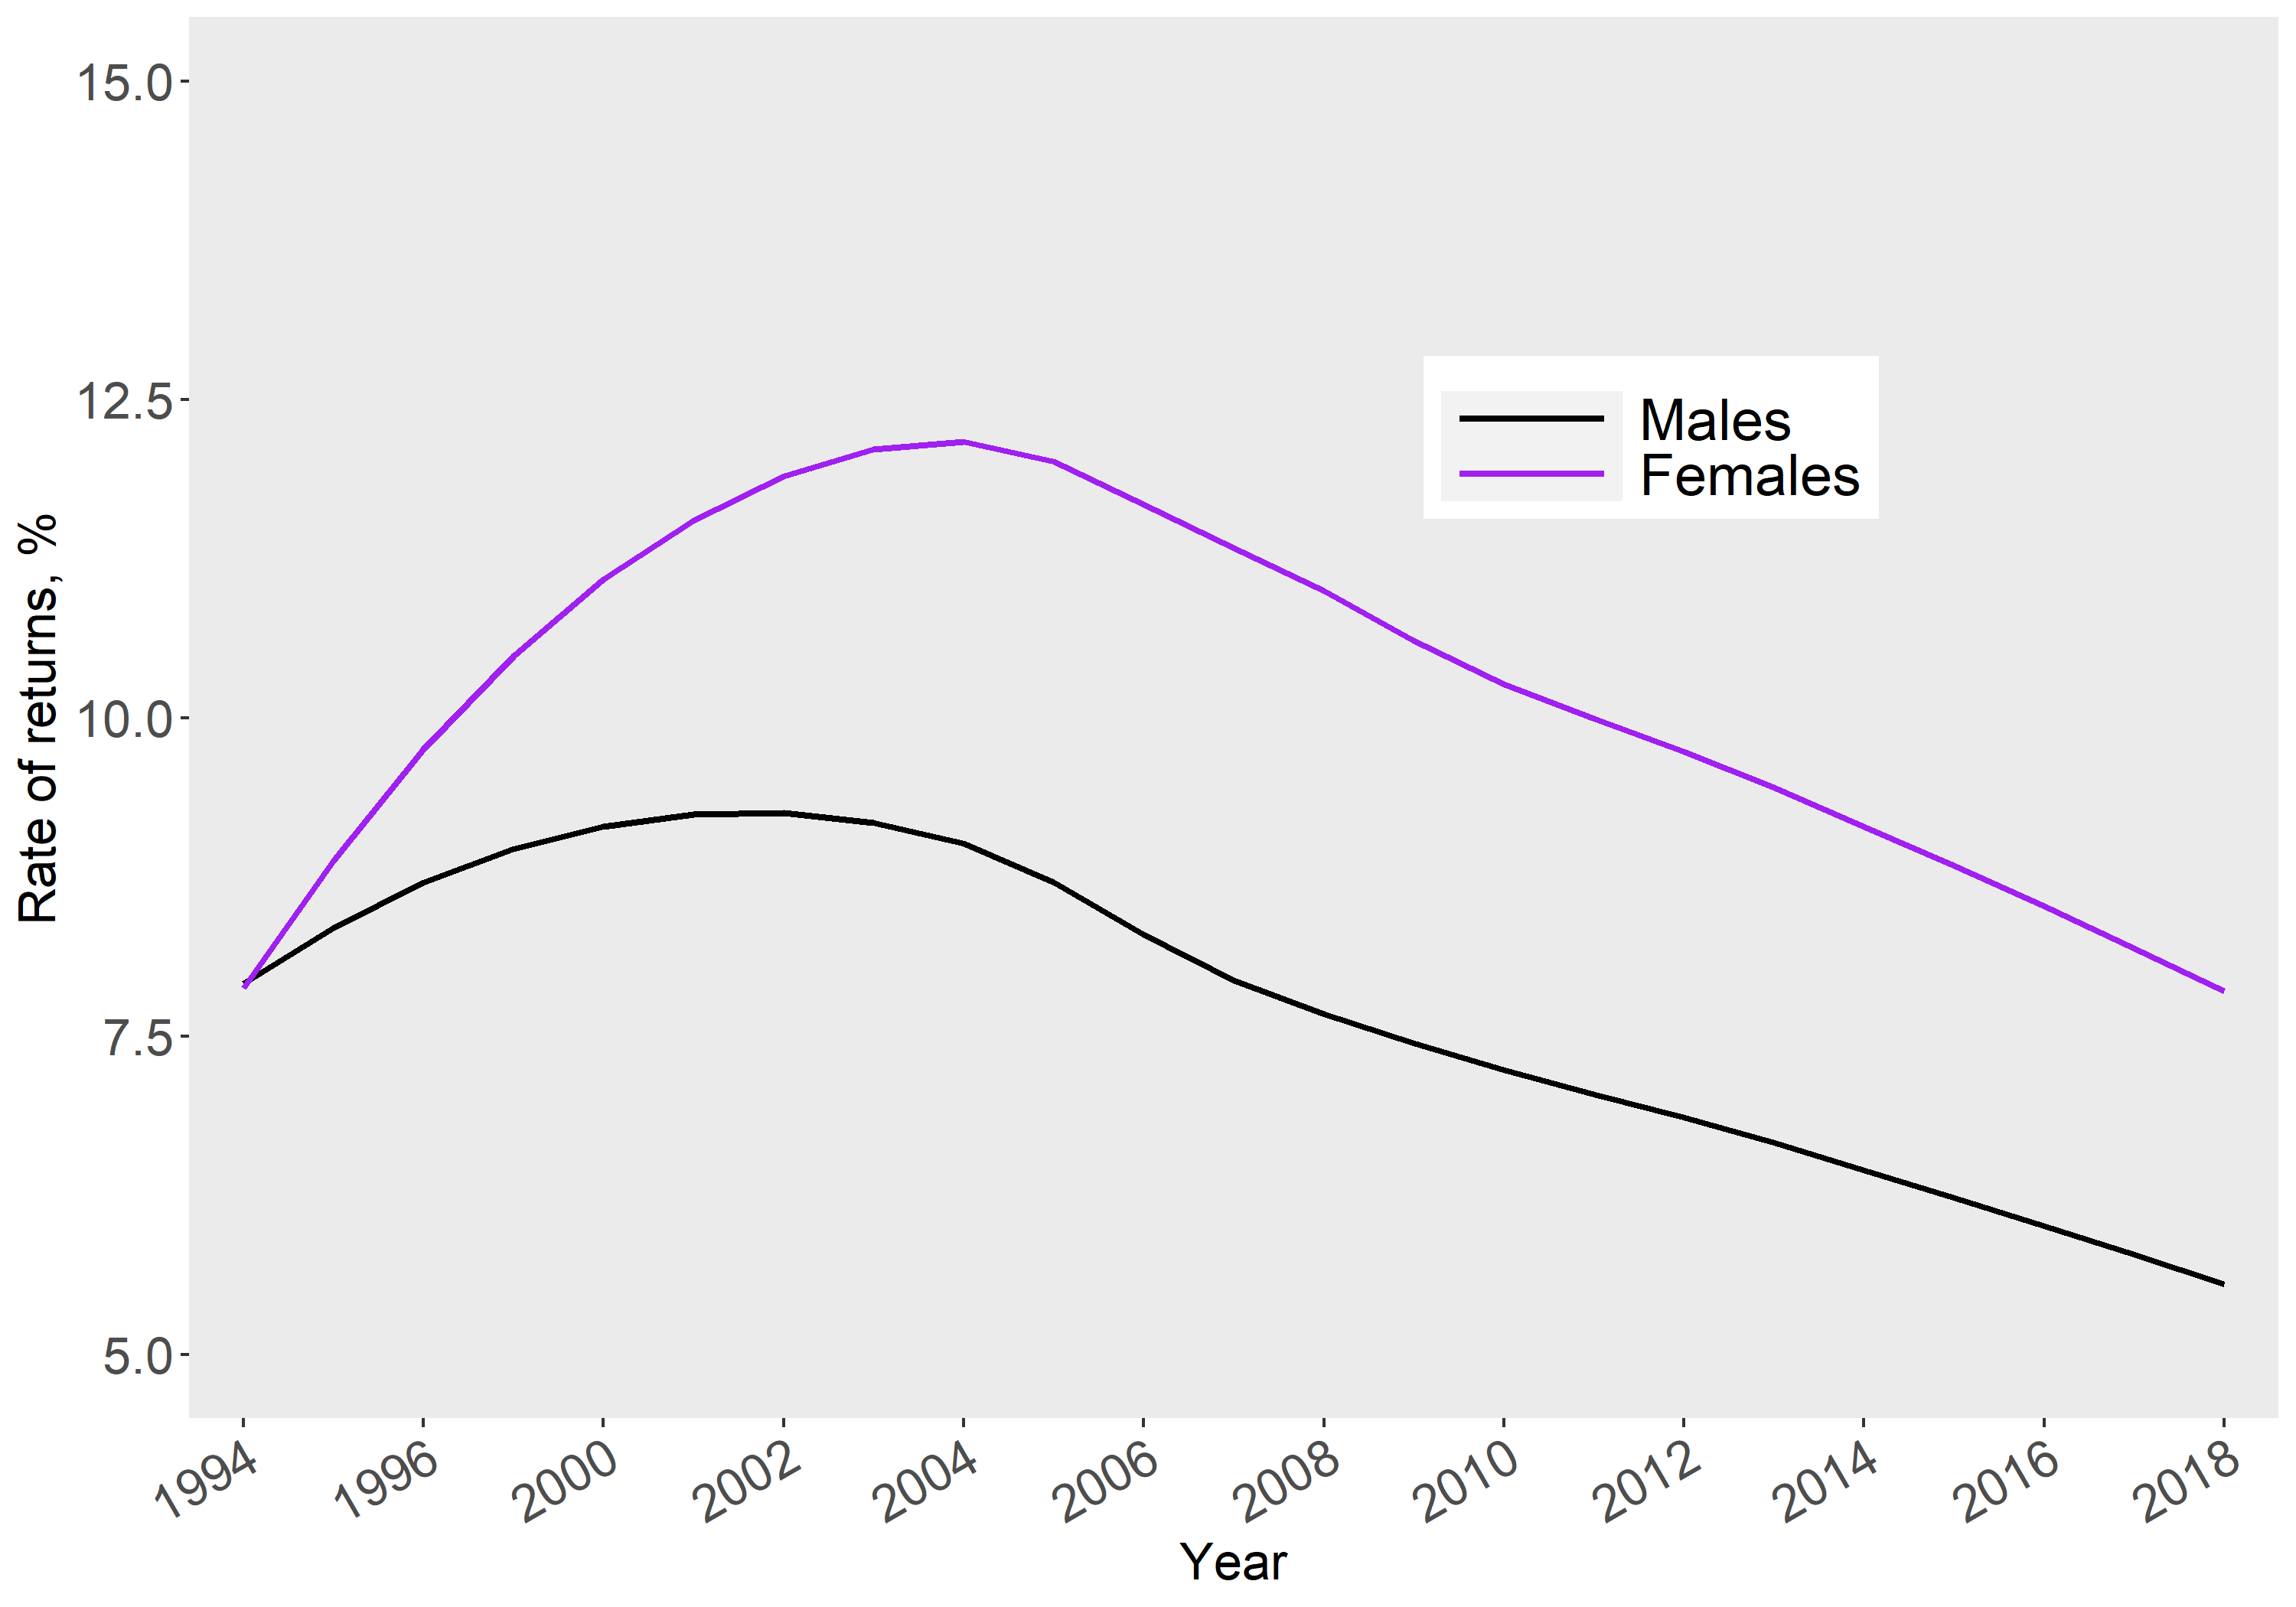
\includegraphics[width=\textwidth, height=275pt]{re_edu2.png}
	\caption{Rates of Returns to Education in Russia, RLMS 
	1994-2018}\label{fig:1.2}
\end{figure}


\hspace{-2em} \textbf{Development policy typology from variations in 
regional context and returns to education}

\vspace{1em}


\noindent A recent World Bank report described the three main factors that 
explain 
the wide scale of diversity in Russia's regions, so that some regions 
have income levels that match Singapore or New Zealand, and others match 
Bolivia or Honduras: (i) the persistent Soviet legacy; (ii) diverse 
physical geography; and (iii) dominance of oil and gas in some regions 
\parencite{worldbank2018}. The report analyzed the determinants of the 
Economic Potential Index (EPI) of Russian regions: urbanization; the 
presence of high-tech industries; advanced human capital; 
and connectivity (access to markets). These four factors explain 60\% of 
the variation in EPI. In this study we create a typology of regions using 
various measures for the quantity and quality of labor demand and supply. 


In this study, we build on the previous research by using an indicator of 
product complexity computed by \cite{lyubimov2018} to define policy context 
for a region. \cite{lyubimov2018} is based on 
a methodology that was initially proposed and implemented by the economists 
Ricardo Hausmann and C\'esar Hidalgo to capture the productive potential 
of an economy on the basis of the diversity of its products and exports 
\parencite{hausmann2011, hausmann2014}. \cite{lyubimov2018} develop an 
``Economic Complexity Index'' (ECI) utilizing production as well as export 
data. Working Paper 3 develops a policy context based on measures of labor 
demand quality and quantity as well as labor supply quality and quantity to 
better situate the differentials in rates of return. The analysis provides 
an opportunity to focus on high priority regions - depicted with red dots 
and their name shown in Figure \ref{fig:4.2}

\setcounter{table}{0}


\begin{figure}[htbp!]
	\begin{minipage}[b]{.5\linewidth}
		\centering
		%\hspace*{-0.2in}
		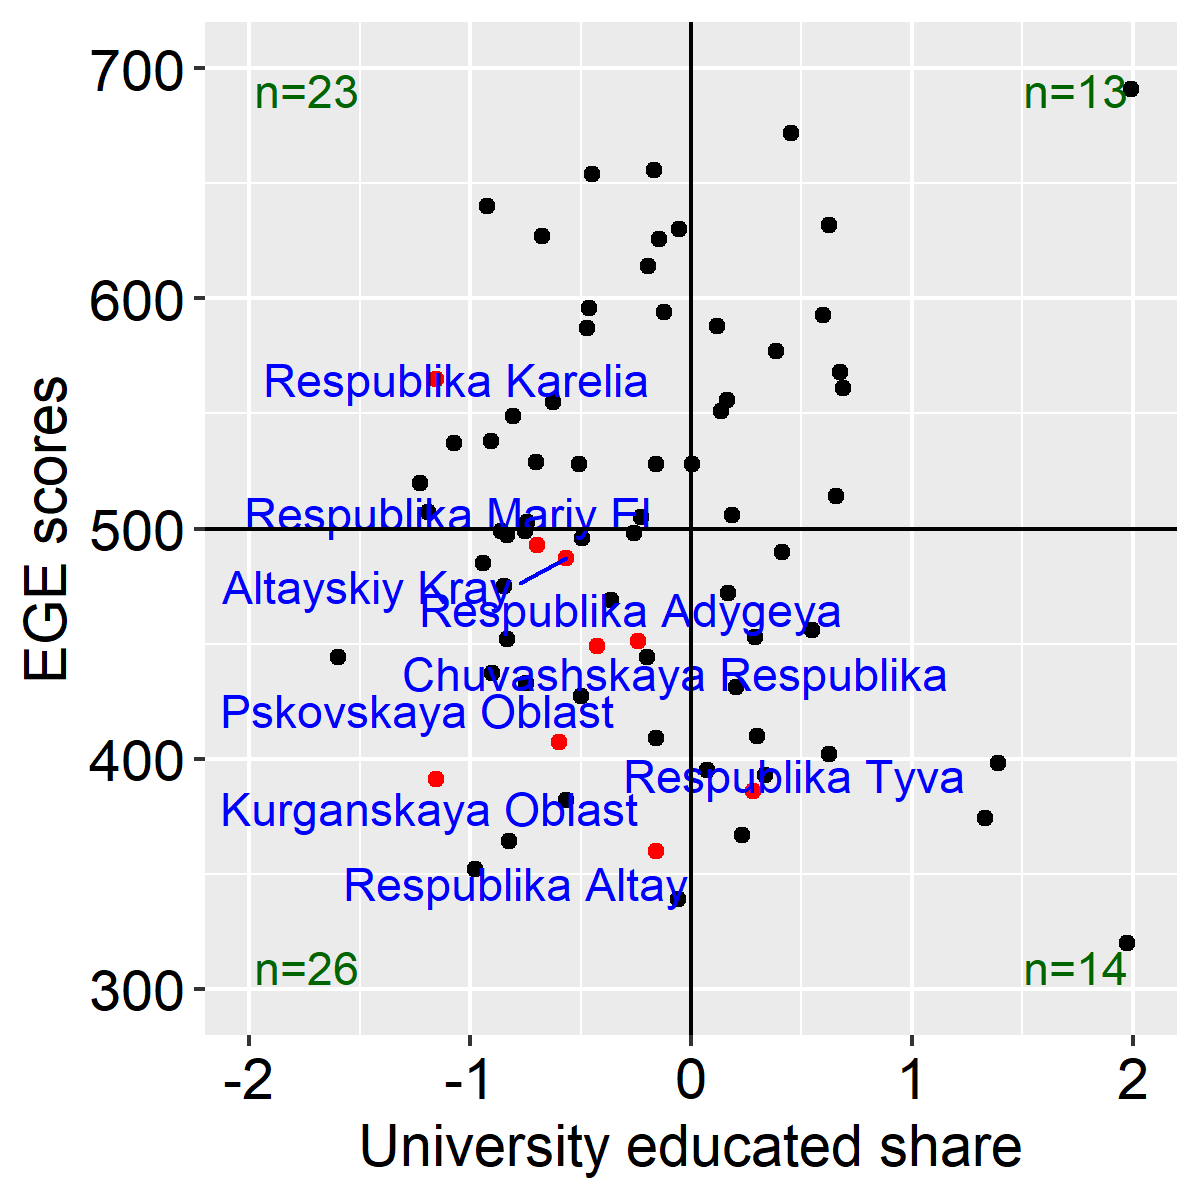
\includegraphics[width=175pt]{ranks1a.png}
		% plot 1
		\subcaption{\large{Labor Supply}}
	\end{minipage}
	\hfill
	\begin{minipage}[b]{.5\linewidth}
		\centering
		%\hspace*{-0.2in}
		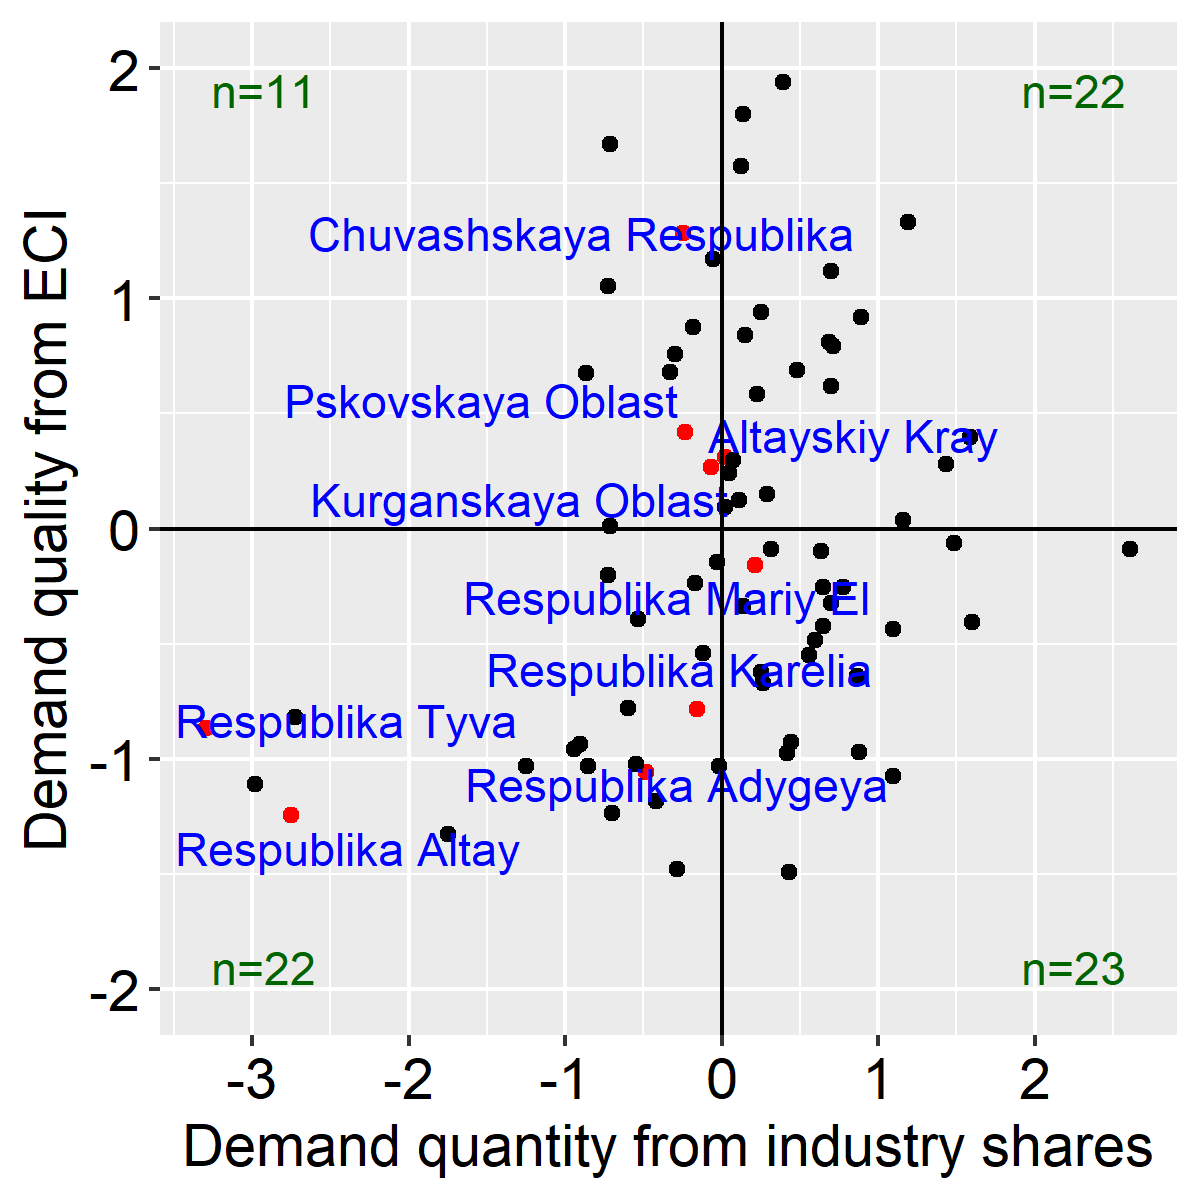
\includegraphics[width=175pt]{ranks1b.png}
		% plot 2
		\subcaption{\large{Labor Demand}}
	\end{minipage}
	\caption{Ranking of Regions on Quantity and Quality 
	dimensions}\label{fig:4.2}
\end{figure}

\hspace{-2em} \textbf{Depreciation detrimentally affects the returns to 
education}

\vspace{1em}

\noindent The study finds deprecation rates of human capital of 2\%. 
Declining 
returns of  education may be an effect of increasing depreciation. Like any 
other form of capital, human capital is also subject to depreciation. The 
literature identifies two kinds of depreciation - one is due to changes in 
technology that renders past learned skills less useful or even obsolete; 
the second is depreciation due to physical or psychological effects of the 
passage of time. Unfortunately, extracting depreciation rates from 
empirical data is not straightforward.


\begin{figure}[htbp!]
	\hspace{0.35in}
	\begin{minipage}[b]{.3\linewidth}
		\centering
		\hspace*{-0.7in}
		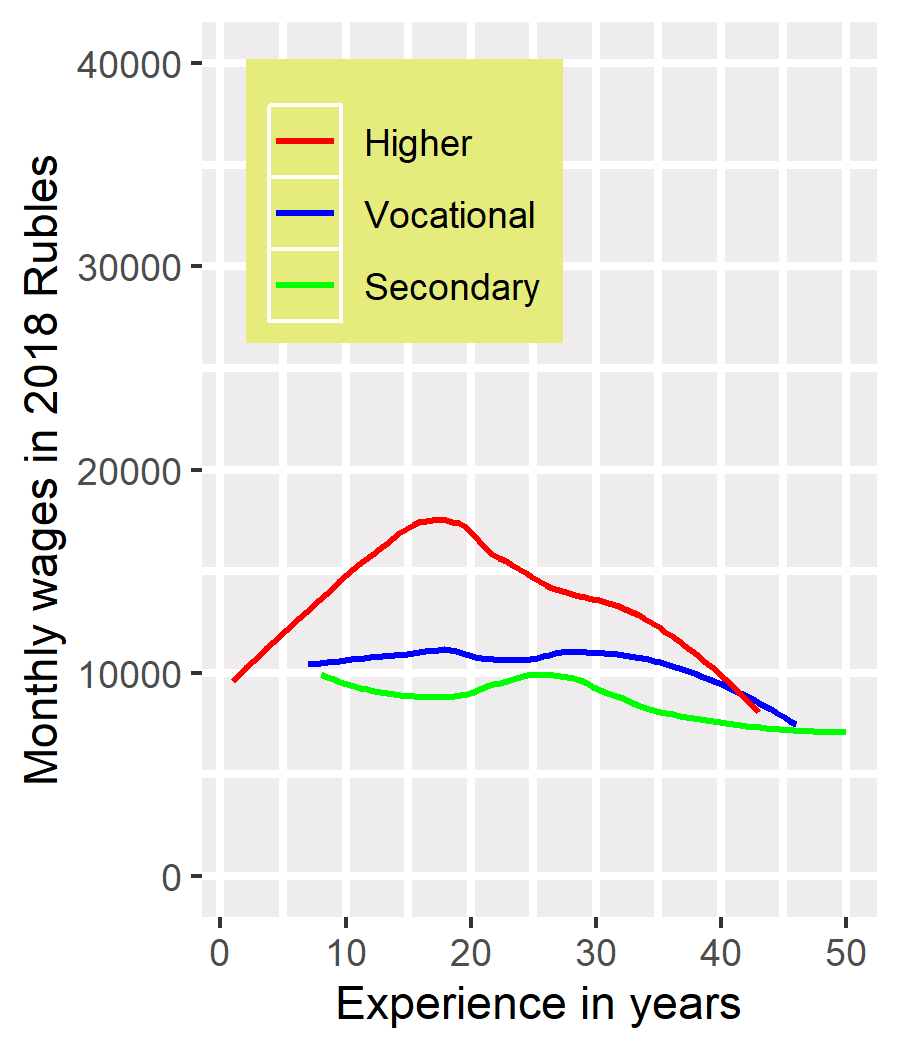
\includegraphics[width=125pt]{dp01_98.png}
		% plot 1
		\subcaption{1998}\label{fig:1.2a}
	\end{minipage}
	\hfill
	\begin{minipage}[b]{.3\linewidth}
		\centering
		\hspace*{-0.7in}
		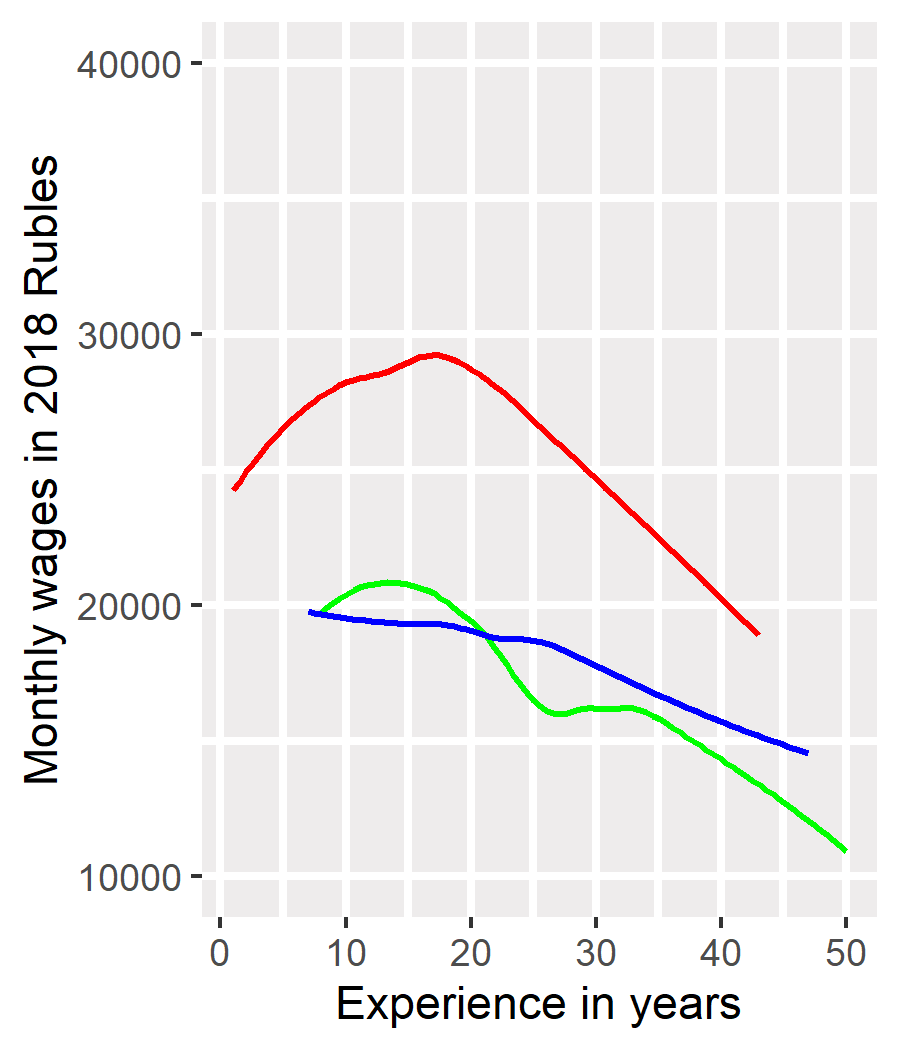
\includegraphics[width=125pt]{dp01_06.png}
		% plot 2
		\subcaption{2006}\label{fig:1.2b}
	\end{minipage}
	\hfill
	\begin{minipage}[b]{.3\linewidth}
		\centering
		\hspace*{-0.7in}
		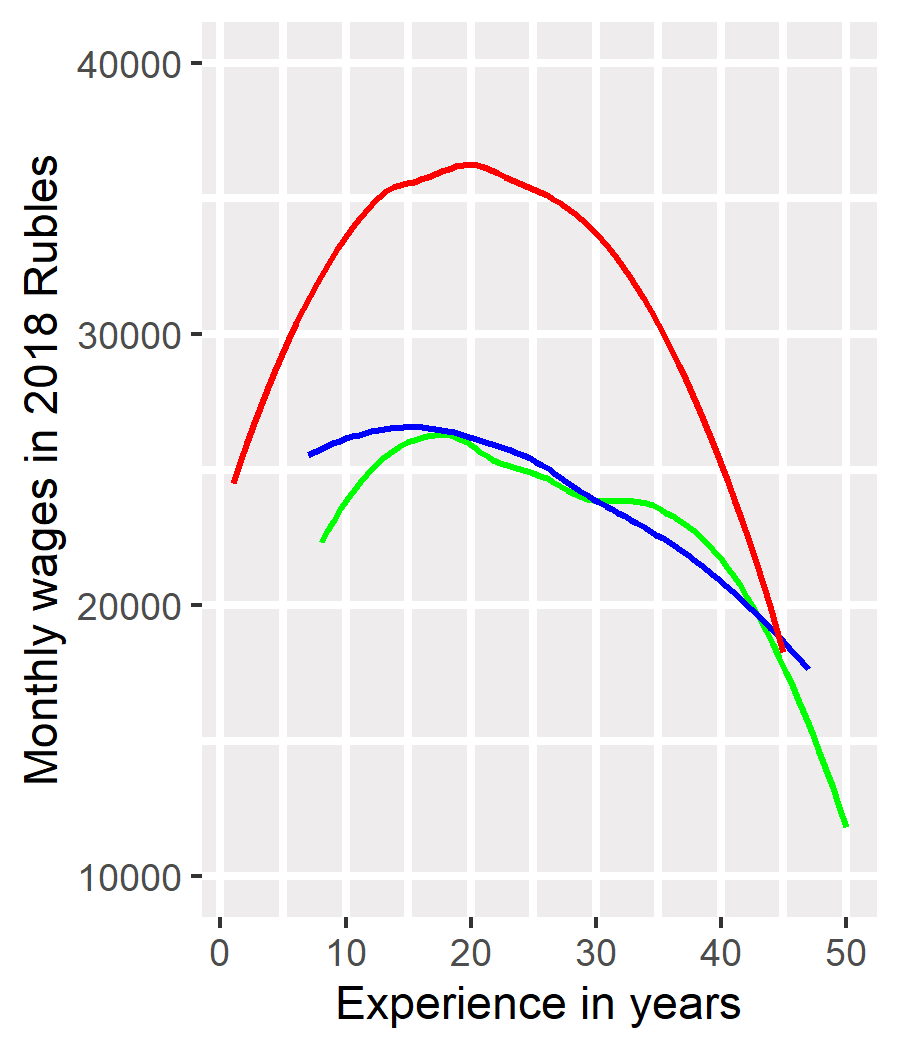
\includegraphics[width=125pt]{dp01_18.png}
		% plot 2
		\subcaption{2018}\label{fig:1.2c}
	\end{minipage}
	\caption{RLMS Rounds 1998, 
		2006 and 2018}\label{fig:1.2}
\end{figure}

 A relatively non-technical or 
intuitive understanding of depreciation can be 
obtained from Figure \ref{fig:1.2}. The trajectory of earnings shows the 
usual 
concave profile for Higher Education. But the profiles for those with 
Secondary Education or Vocational education has a very early peak. 
Depreciation can be stemmed through  
repeated or regular human capital investment through a worker's lifetime. 
Some of the European countries including Denmark and Norway have developed 
strong lifelong learning systems 
\parencite{jorgensen2007,midtsundstad2019}. 

\newpage

\hspace{-2em} \textbf{Institutional Level Fiscal and Private Returns to 
Education}

\vspace{1em}

\noindent \url{Graduate.edu.ru} is the official graduate employment 
monitoring portal 
created and maintained by the Ministry of Education of the Russian 
Federation. The website was launched in 2015 to provide information 
targeted mainly to prospective graduates about the employment record of 
graduates from tertiary education institutions - including universities and 
vocational education colleges. The \url{bus.gov.ru} website is the official 
website of the Russian Federation for provision of information by public 
institutions. The objective as stated on the website is ``to increase the 
openness and accessibility of information about state (municipal) 
institutions, as well as about their activities and property''. 

In Working Paper 4 of this study, the information from the two websites is 
merged to provide early stage fiscal and private returns to education.  
Information is available for the total annual revenue from different 
sources including government transfers and grants, as well as revenue from 
service payments made by private individuals. For education institutions 
(colleges and universities) we assume that the revenues from service 
payments are tuition fee payments. The very short period of earnings 
information available (only 3 years) Table \ref{tab:1.3} shows 
that the most profitable educational investments, albeit with a three year 
horizon, may not always be the most famous ones! 


Combining the costs and benefits side of investment in education will be 
useful not just for  individual students but also for overall system 
efficacy and efficiency.  Though multi-dimensional rankings are popular in 
some policy circles, transparent and simple fiscal and private returns 
would spur healthy competition between institutes and regions to attract 
the best students. 


\begin{table}[htbp!]
	\def\arraystretch{0.8} 
	%\setlength\arrayrulewidth{1pt}
	\centering
	\caption{Fiscal and Private Returns by Institution: Top and Bottom 10}
	\label{tab:1.3}
	\begin{tabular}{|p{.75cm}|p{.75cm}|p{7cm}|p{3cm}|R{1.25cm}|}
		\hline
		\multicolumn{5}{|c|}{\textbf{Top 10 Colleges}} \\ \hline
		fiscal  & private  & Name & Region  & Number graduates\\ \hline
		0.13 & 0.35 & Samara Power Engineering College & Samarskaya Oblast 
		& 140 \\ 
		0.13 & 0.22 & Tomsk Polytechnic Technical School & Tomskaya Oblast 
		& 306 \\ 
		0.12 & 0.24 & Novocherkassk Geological Exploration College & 
		Rostovskaya Oblast & 244 \\ 
		0.12 & 0.28 & Vilyui Technical School & Resp. Sakha (Yakutia) & 156 
		\\ 
		0.11 & 0.21 & Kiselevsky Mining College & Kemerovskaya Oblast & 280 
		\\ 
		0.11 & 0.25 & Higher Banking School & Saint-Petersburg & 229 \\ 
		0.11 & 0.24 & Industrial and Technological College & 
		Saint-Petersburg & 305 \\ 
		0.10 & 0.18 & Perm Oil College & Permskiy Krai & 171 \\ 
		0.10 & 0.30 & Yakut Road Technical School & Resp. Sakha (Yakutia) & 
		220 \\ 
		0.10 & 0.19 & Sakhalin Indus. \& Economic College & Sakhalinskaya 
		Oblast & 489 \\ 
		-0.01 & 0.01 & Tomsk Industrial University & Tomsk & 6655 \\ \hline 
		\multicolumn{5}{|c|}{\textbf{Top 10 Universities}} \\ \hline
		fiscal  & private  & Name & Region  & Number graduates \\ \hline
		0.07 & 0.09 & Buryat State Agricultural Academy & Respublika 
		Buryatia & 415 \\ 
		0.05 & 0.09 & Russian State Univ. of Tourism and Service & 
		Moskovskaya Oblast & 3019 \\ 
		0.05 & 0.07 & Tyumen Industrial University & Tyumenskaya Oblast & 
		6655 \\ 
		0.04 & 0.07 & Samara State Univ. of Economics & Samarskaya Oblast & 
		1826 \\ 
		0.04 & 0.20 & North-Eastern State University & Magadanskaya Oblast 
		& 573 \\ 
		0.04 & 0.10 & Siberian State Industrial University & Kemerovskaya 
		Oblast & 1727 \\ 
		0.04 & 0.13 & Samara State Technical University & Samarskaya Oblast 
		& 2879 \\ 
		0.03 & 0.09 & Siberian State Univ. of Geosystems \& Technologies & 
		Novosibirskaya Oblast & 1768 \\ 
		0.03 & 0.10 & Kamchatka State Technical University & Kamchatskaya 
		Kray & 826 \\ 
		0.02 & 0.15 & Arctic State Inst. of Culture and Arts & Resp. Sakha 
		(Yakutia) & 366 \\ 
		\hline
	\end{tabular}
\end{table}



\newpage

\section{Future Areas of Inquiry}



Empirical research to inform policy is necessarily tightly bound by time 
constraints. Some of the lines of inquiry that can be explored further are 
mentioned here. Particularly useful would be support to regional 
development strategies and their implementation, for instance with regard 
to the priority regions whose development is directly tied to the 
attainment of ambitious national development goals. The following future 
areas of inquiry are suggested:


\begin{itemize}
	
\item \textbf{Causal Effects of Educational Investments} Causal marginal 
effects of education on earnings can be computed
\parencite{carneiro2011,heckman2018}. This has been done recently for the  
Russian Federation, in an academic study that explored the marginal effect 
of the expansion of university education in the 2000s 
\parencite{belskaya2020}. In an upcoming 
seminar where this study will be presented in June, 2020 another researcher 
will present a paper on the causal effect of the shift in Russian 
universities to the Bologna accord \parencite{avdeev2020}. More recently 
developed machine learning techniques hold great promise and can be applied 
to regional returns in the Russian Federation \parencite{kim2019}. 
	
\item \textbf{Detailed Institutional Returns} In a competitive higher 
education global environment, countries have set up detailed databases 
regarding the cost of education, for example 
\url{https://www.hesa.ac.uk/data-and-analysis} in the UK and 
\url{https://nces.ed.gov/ipeds/} in the USA. The bus.gov.ru database, while 
not established for that purpose, has provided a useful starting point as 
demonstrated in this study. A staged research study that collects further 
information from the institutes themselves would be very useful. Also, with 
adequate safeguards to protect privacy, household surveys conducted by 
Rosstat could begin to record the identity of the institution where an 
individual study. An online platform can be created with a feedback system 
to ensure data accuracy and transparency. 

\item \textbf{Entrepreneurship and Returns} There is a very interesting 
variable in the graduate.edu.ru website that was not exploited in the study 
- this is information about graduates who are registered with the Pension 
Fund as entrepreneurs, together with information about their earnings. 
Traditionally, entrepreneurs may not have been well represented in studies 
of returns to education because of their often sporadic income. However, 
Russia's future prosperity hinges on the creation of new jobs and through 
innovation - it would be extremely useful to study how entrepreneurs fare 
in terms of earnings, and the causal effect of their education.

\item \textbf{Regional Efficiency} Fiscal returns to education by region 
have been provided in this study as a first approximation based on data 
that is available regarding costs for a six year period from 2013 to 2018. 
The effective subsidization of college and university education can be 
evaluated very well by examining the divergence between private and fiscal 
returns. The analysis can also be disaggregated by specialization, spatial 
categories or by administrative arrangements. With regions seeking to 
accelerate their development, fiscal efficiency is particularly important 
and studies building further on the demonstrated example of this study can 
be deployed for that purpose. 

\item \textbf{Effect of Covid-19} Four kinds of 
studies regarding the impact of the Covid-19 related shutdowns with the 
purpose of mitigation and to develop resilience 
to future pandemics: (a) Impact of lost time in education on learning or 
cognitive achievement of children and youth; (b) Impact of truncation of 
schooling year on eventual educational attainment; (c) Positive deviance 
studies regarding digital or distance education that worked or other 
factors that provided resilience to learning loss \parencite{pascale2010}; 
(d) Simulation studies of potential impacts of learning loss on economic 
output in the future. 
	
\end{itemize}

\newpage

\section{Five Main Recommendations}

\textbf{Education quality and innovation policy:} The 
Russian Federation needs to make investments in the quality of education 
and enhance youth entrepreneurship to stem the tide of falling returns to 
education. It appears very difficult for state owned enterprises or the 
public sector to generate bigger streams of job openings and also become 
more efficient. Quality improvements in education, geared to providing 
students with `learning to learn skills' as well as practical skills such 
as financial literacy, with continued improvements in `Doing Business' 
indicators will lead to productivity improvement. 
\vspace{0.4em} 

\hspace{-1.8em} \textbf{Policy needs to work harder for gender parity:} 
Gender segregation of jobs and gender earning gaps remain wide in the 
Russian Federation, with women earning lower than men at all levels of 
education. Returns to education have been higher for women which would help 
to reduce the gap, but recent data indicates that women may have stopped 
going to university in the numbers they were doing before, which does not 
bode well for the earnings gap. Policies to retain women's interest in 
university education and provision of learning opportunities at work will 
help to resume the path towards gender parity in earnings.   

\vspace{0.4em} 

\hspace{-1.8em} \textbf{Lifelong learning for vocational education:} 
Supporting continuous investment in human capital through the career is 
more important now the base level of education in Russia is amongst the 
highest in the world; this will reduce depreciation, especially for 
vocational education. Reduction in the depreciation of human capital will 
help to improve the returns to education. Depreciation can be reduced not 
only through learning while on the job, but also by the content and method 
of schooling so that students become proficient lifelong learners. 

\vspace{0.4em} 

\hspace{-1.8em} \textbf{Strategy for priority regions:} A policy 
diagnostic based even  on rough measures of labor market demand and supply 
is shown to capture  regional diversity. Refinement of the measures for the
high priority regions will support the design of customized policy 
solutions, for example for three pilot regions of Pskov Oblast, Altai Krai, 
and the Adygea Republic. Human capital formation tends to have long 
historic roots and path dependence means that regions similar in terms of 
gross regional product may have vastly different human capital potential 
and challenges. 

\vspace{0.4em} 

\hspace{-1.8em} \textbf{Government transparency for citizen benefit:}. 
Revitalize the  \href{https:\\graduate.edu.ru}{graduate.edu.ru} website 
which has not  been updated since 2016; Deepen the financial information 
collected from  \href{https:\\bus.gov.ru}{bus.gov.ru} and annually update 
resulting data on  institution level education returns to 
improve student choice and system efficiency. Collecting accurate 
information on graduate salaries and on college and university costs is 
itself a costly endeavor, but is amply justified by the gains in efficiency 
that would result. The transparency and digital government initiatives 
undertaken by the Government have been progressive, but are not yet 
instrumental in meeting strategic development goals. To be truly effective, 
a further set of steps need to be made, to close the feedback loop with 
citizens making decisions based on the information provided, and those 
decisions, in turn, influencing institutional and system management. 

\newpage
\printbibliography

\end{document}
